\section*{سوال 4}
\begin{enumerate}
    \item \lr{overfitting} بدین معنا است که درجه‌ی مدلمان را بسیار زیاد گرفتیم و مدل عملا آن‌طور که باید
    خودش را نشان نمی‌دهد. به عنوان مثال به شکل
    \ref{fig:overfit}
    که از اسلاید‌ها برداشته شده است توجه کنید.
    \begin{figure}[H]
        \centering
        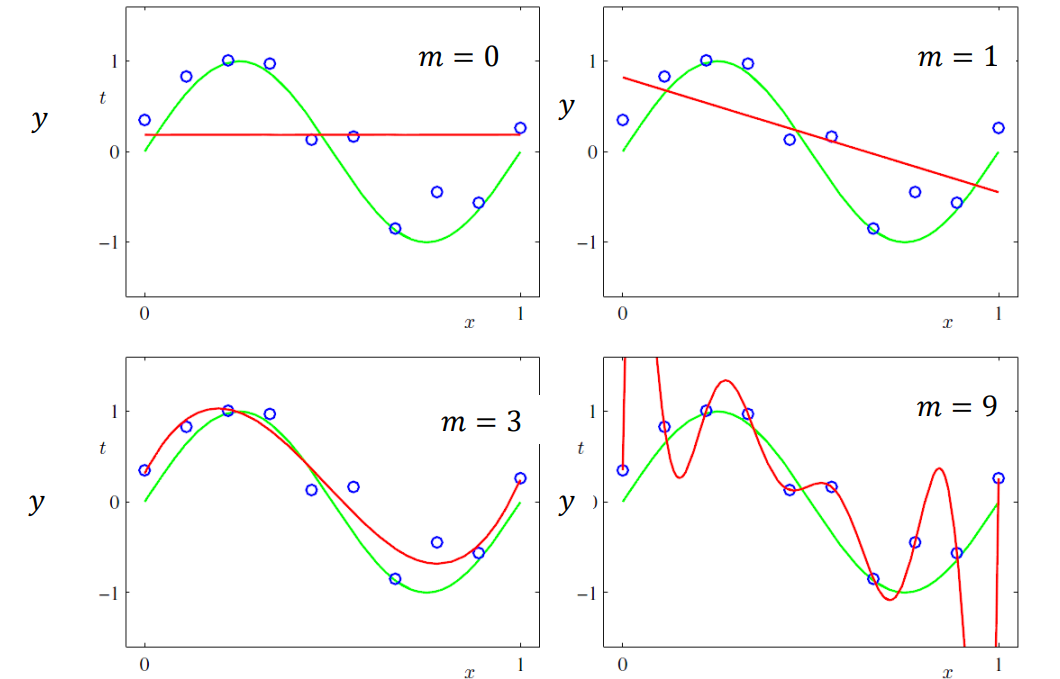
\includegraphics[scale=0.5]{pics/overfit.png}
        \caption{نمونه‌ای از \lr{overfitting} و \lr{underfitting}}
        \label{fig:overfit}
    \end{figure}
    در این شکل نمودار پایین سمت راست مصداق
    \lr{overfit}
    است. بدین منظور که اینقدر که درجه را زیاد کردیم که با اینکه نمودار از روی نقاط
    \lr{training set}
    رد می‌شوند ولی در صورتی که چشمی نگاه کنیم متوجه می‌شویم که نمودار درست نیست.
    \lr{Underfitting}،
    دقیقا برعکس نشان می‌دهد که اینقدر نمودار ساده است که از روی تمامی نقاط رد نمی‌شود و همچنین خطای زیادی دارد.
    مانند شکل بالا چپ.
    \item زمانی که پیچیدگی مدل کم است، هم خطای
    \lr{training model}
    زیاد است و هم خطای
    \lr{validation model}.
    دلیل این موضوع این است که مانند شکل سمت بالا چپ
    \ref{fig:overfit}
    اصلا نمودار از روی نقاط نمی‌گذرد که بخواهد دقیق باشد! پس خطای جفت آنها زیاد است.
    قسمت آخر نمودار وقتی که
    \lr{model complexity}
    را زیاد می‌کنیم، مشکل
    \lr{overfitting}
    رخ می‌دهد. با اینکه خود نمودار خیلی نزدیک به نقاط است ولی در دیتای واقعی جواب‌های پرت می‌دهد.
    به همین منظور به نظرم نمودار وسطی بهتر و منطقی تر است.
\end{enumerate}